\documentclass[a4paper]{article}
\usepackage[utf8]{inputenc}
\usepackage[L7x]{fontenc}
\usepackage[lithuanian]{babel}
\usepackage{lmodern}
\usepackage{graphicx}
\usepackage[top=2cm, bottom=2cm, left=1.5cm, right=1.5cm, footskip=1cm, a4paper]{geometry}
\usepackage{indentfirst}
\usepackage{framed}
\usepackage{tikz}
\usepackage{listofitems}
\usepackage{xcolor}
\usepackage{verbatim}
\usepackage[unicode]{hyperref}
\usepackage{amsmath,amsfonts,amssymb,amsthm}
\usepackage{minted}
\usepackage{cancel}
\usepackage{framed}
%\usepackage{mathptmx}
\usepackage{calc}
\usepackage{tasks}
\usetikzlibrary{tikzmark,calc,,arrows,shapes,decorations.pathreplacing}
\tikzset{every picture/.style={remember picture}}
\usepackage{accents}
\newcommand\myubar[1]{%
\underaccent{\bar}{#1}}
\graphicspath{{"/Users/Vartotojas/Desktop/EnolaProject/Kodinimas/Pythoning/demo - create folder of images problems in pdf/"}}
\renewenvironment{framed}[1][\hsize]
   {\MakeFramed{\hsize#1\advance\hsize-\width \FrameRestore}}%
   {\endMakeFramed}

\newcommand{\inc}[1]{\includegraphics[width=\textwidth]{#1}}
\newcommand{\goto}[2]{\href{\detokenize{#1}}{\textcolor{blue}{#2}}}
\newcommand{\say}[1]{\textbf{\textit{#1}}}
%use python script:
%lines='''B2002_5, B2002_4'''
%print(', '.join([n[1:5]+'/'+n[0:5]+'/'+n+'.jpg' for n in lines.replace(" ", "").split(',')]))
\begin{document}
\subsection*{Rekordinis pasaulio priartinimas}
\say{Aš}. Šią pamoką, kiek mums pavyks, norėčiau papasakoti apie procesus, kurie vyksta mikroskopinėje erdvėje: ląsteles, chromosomas, DNR, molekules ir atomus. Galėčiau parodyti, kaip reiktų kelti klausimus, susirasti reikiamą informaciją ir kokių prireikia skaičiavimų norint atsakyti į tam tikrus klausimus. Mūsų mikroskopinio pasaulio nagrinėjimas turėtų prasidėti nuo šio \goto{https://www.youtube.com/watch?v=7WhRJV_bAiE}{filmuko}.

\say{Simonas}. Žiūrėk, ir aš noriu kai ką parodyti. Praeitą savaitę pamačiau patį galingiausią mikroskopą. Ar galiu parodyti šį \href{https://www.youtube.com/watch?v=zXTpASSd9xE\&t=101s}{\textcolor{blue}{video}}?. 

\say{Aš}. Kaip manai, kiek šis mikroskopas kartų gali padidinti daiktus?

\say{Simonas}. Nežinau, manau milijoną.

\say{Aš}. Neteisingai. Nuorodoje matyti du skaičiai: $10^{198}$ ir $350000000$ iterations. Pirmasis reiškia, kiek kartų didiname, antrasis - kiek perskaičiavimų reikėjo daryti. Padidinę milijoną kartų žmogaus plauką, mes galėtume pamatyti keratino - baltymo, iš kurio jis sudarytas - molekulę. Ji yra taip pat plona ir ilga, kaip plaukas, tačiau 50000 kartų už jį plonesnė. O jei padidintume milijoną kartų, pamatytume sieros, deguonies, azoto ir anglies atomus, kurių skersmuo yra trumpesnis už plauko skersmenį nuo milijono iki dviejų milijonų kartų. Tačiau milijonas yra skaičius, turintis vienetą su šešiais nuliais, kai tuo tarpu šiame video atliekamas padidinimas skaičiumi, kuris turi vienetą su 198 nulių. Ar žinai, kas čia didinama?

\say{Simonas}. Ne.

\say{Aš}. Tai kaip gali sakyti, jog čia rekordas? Reikia išsiaiškinti. Video pavadinimas yra \textit{Malderbrot zoom}. Kas tai yra? Kaip sužinoti?

\say{Simonas}. Neįsivaizduoju.

\say{Aš}. Iš tiesų, tai mes žinome, ką reiškia \textit{zoom}. Bet nežinom, ką reiškia \text{Malderbrot}. Reikia nukopijuoti ir įvesti tai į Google. Išmeta \goto{https://en.wikipedia.org/wiki/Mandelbrot_set}{nuorodą} į anglišką Vikipediją su tokiu apibrėžimu:

\begin{center}
\textit{The Mandelbrot set is the set of complex numbers $\displaystyle c$ for which the function $\displaystyle f_{c}(z)=z^{2}+c$  does not diverge when iterated from $z=0$, i.e., for which the sequence $0,f_{c}(0), f_{c}(f_{c}(0))$, etc., remains bounded in absolute value.}
\end{center}

Ar aiškiau?

\say{Simonas}. Ne.

\subsection*{Aibės ir fraktalai}
\say{Aš}. Tad reikia žiūrėti, kokius žodžius suprantame ir kokius ne. Ar aišku, kas yra aibė?

\say{Simonas}. Taip, tai gali būti keleto skaičių rinkinys.

\say{Aš}. Gerai. O ar ji gali būti begalinė?

\say{Simonas}. Taip, pavyzdžiui realieji skaičiai.

\say{Aš}. Matau, kad suprasti sekasi visai neblogai. Pradžiai reikėtų patyrinėti įdomesnes aibes. Pavyzdžiui \goto{https://en.wikipedia.org/wiki/Cantor_set}{Kantoro aibę}. Ji yra sudaroma pradžioje paimant atkarpą (tarkim einančią nuo 0 ligi 1). Ir ties kiekvienu žingsniu visose gautose atkarpose išimant po vidurį. Tą atliekant be galo daug kartų paaiškėja, kad gautoje atkarpoje visai neliko taškų. Pavyzdžiui nuorodęs skaičių 0,32 aš iš karto žinau, kad taško, nutolusio nuo atkarpos pradžios per 0,32 toje aibėje nebus. Kaip ir bet kurio kito taško. Kaip taip gali būti?

\say{Simonas}. Nesuvokiama. 

\say{Aš} Nuorodoje matome, kad sulig kiekvienu žingsniu atkarpoje lieka vis daugiau tuščios erdvės. Tai atlikus kiek nori daug išėmimų atkarpoje tiesiog nieko neliks. Bet pabandykime tokius sumažėjimus suvokti dar giliau. Tam patyrinėkime \goto{https://en.wikipedia.org/wiki/Koch_snowflake}{Kocho snaigę}. Tai yra baigtinio ploto ir begalinio perimetro geometrinė figūra. Ar aišku, kaip kinta šios figūros perimetras sulig kiekvienu žingsniu?

\say{Simonas}. \textit{Bando skaičiuoti. Iš pradžių mano, kad iš 3 virsta į 9. Po to paaiškėja, kad iš tiesų ties antru žingsniu yra ne 9, o 12 sienelių - kiekvienai antros žvaigždės viršūnei iš 6 turi būti po dvi sieneles. Vėliau Simonui reikia priminti, kad darant pakeitimą iš ,,\_\_\_'' į ,,\_/$\backslash\_$ '' gautos kreivės ilgis niekaip negali iš 1 pavirsti 4. Pamatęs savo klaidą Simonas spėja, kad naujos atkarpos ilgis bus 1,5. Tačiau teisingas atsakymas turėjo būti $\frac{4}{3}$. Čia atsiranda naujos problemos. Reikia suprasti, jog atkarpos ilgį yra įmanoma padidinti ne tik 2 ar 5 kartus, bet taip pat ir $\frac{4}{3}$ karto. Simonas žino, kad norint padauginti skaičių iš $\frac{4}{3}$ reikia padalyti iš 3 ir padauginti iš 4, tačiau su atkarpomis to dar nėra daręs. Suvokti, kad kiekvieną žvaigždės kraštą pakeitus į kreivę, kurios ilgis yra $\frac{4}{3}$ karto didesnis, perimetras taip pat padidės $\frac{4}{3}$ karto, užtrunka šiek tiek laiko}.

\say{Aš}. Tad išsiaiškinom, kad sulig kiekvienu žingsniu naujos žvaigždės perimetras padidėja $\frac{4}{3}$ karto. Taigi, jei jis iš pradžių buvo lygus $1$, tai po to bus jau $\frac{4}{3}$. O koks bus dar po to?

\say{Simonas}. Gal $\frac{8}{6}$?

\say{Aš}. Tai juk reikia prisiminti, ką reiškia perimetrą, kurio dydis yra $\frac{4}{3}$ padidinti dar $\frac{4}{3}$ karto. 

\say{Simonas}. A, tai tada $\frac{16}{9}$?

\say{Aš}. Teisingai. Beveik 2. O kaip su kitais perimetrais? 

\say{Simonas}. Po to dauginti dar iš $\frac{4}{3}$. 

\say{Aš}. Gerai. Tai bus $\frac{64}{27}$ Jau virš 2. Gal reiktų pabandyti atspausdinti pirmuosius 100 rezultatų. \textit{Atsiverčiu Python ir rašau kodą} (trunka apie minutę):
\begin{minted}{python}
k=4/3
for i in range(1,101): print(i, k); k*=4/3
\end{minted}
Bet geriau rašyti šitaip:
\begin{minted}{python}
k=4/3
for i in range(1,101): 
    print(i, k)
    k*=4/3
\end{minted}
Rezultatas:

\begin{tabular}{|r|l|}
\hline
1 & 1.3333333333333333\\ \hline
2 & 1.7777777777777777\\ \hline
3 & 2.3703703703703702\\ \hline
4 & 3.1604938271604937\\ \hline
5 & 4.213991769547325\\ \hline
6 & 5.6186556927297655\\ \hline
7 & 7.491540923639687\\ \hline
8 & 9.988721231519582\\ \hline
9 & 13.318294975359443\\ \hline
10 & 17.757726633812588\\
\vdots & \vdots \\
98 & 1753865105741.9583\\ \hline
99 & 2338486807655.9443\\ \hline
100 & 3117982410207.926\\ \hline
\end{tabular}

\say{Pastaba:} Simonas kodą gali nukopijuoti į \href{http://pythontutor.com/visualize.html\#mode=edit}{\textcolor{blue}{Online interpretatorių}} ir stebėti, kas vyksta atskiruose programos veikimo žingsniuose.

\say{Aš}. Kaip manai, kokie bus tolimesni rezultatai?

\say{Simonas}. Artės į begalybę.

\say{Aš}. Teisingai. O gal žinai, kaip greit gauti šimtąjį narį?

\say{Simonas}. Reikėtų $\frac{4}{3}$ pakelti šimtuoju laipsniu.

\say{Aš}. Taip, viskas teisingai. Gavome, kad rezultatas artėja į begalybę. Vadinasi, figūros perimetras bus begalinis. O plotas, kaip matome, ne.

\say{Simonas}. Parodyk \href{https://en.wikipedia.org/wiki/Koch_snowflake\#Variants_of_the_Koch_curve}{\textcolor{blue}{čia žemiau}}. Aš esu matęs tą kreivę, kur ketvirtoj eilutėj.

\say{Aš}. Taip, aš irgi ją braižydavau. Štai čia yra mano mokyklinių laikų sąsiuvinis:

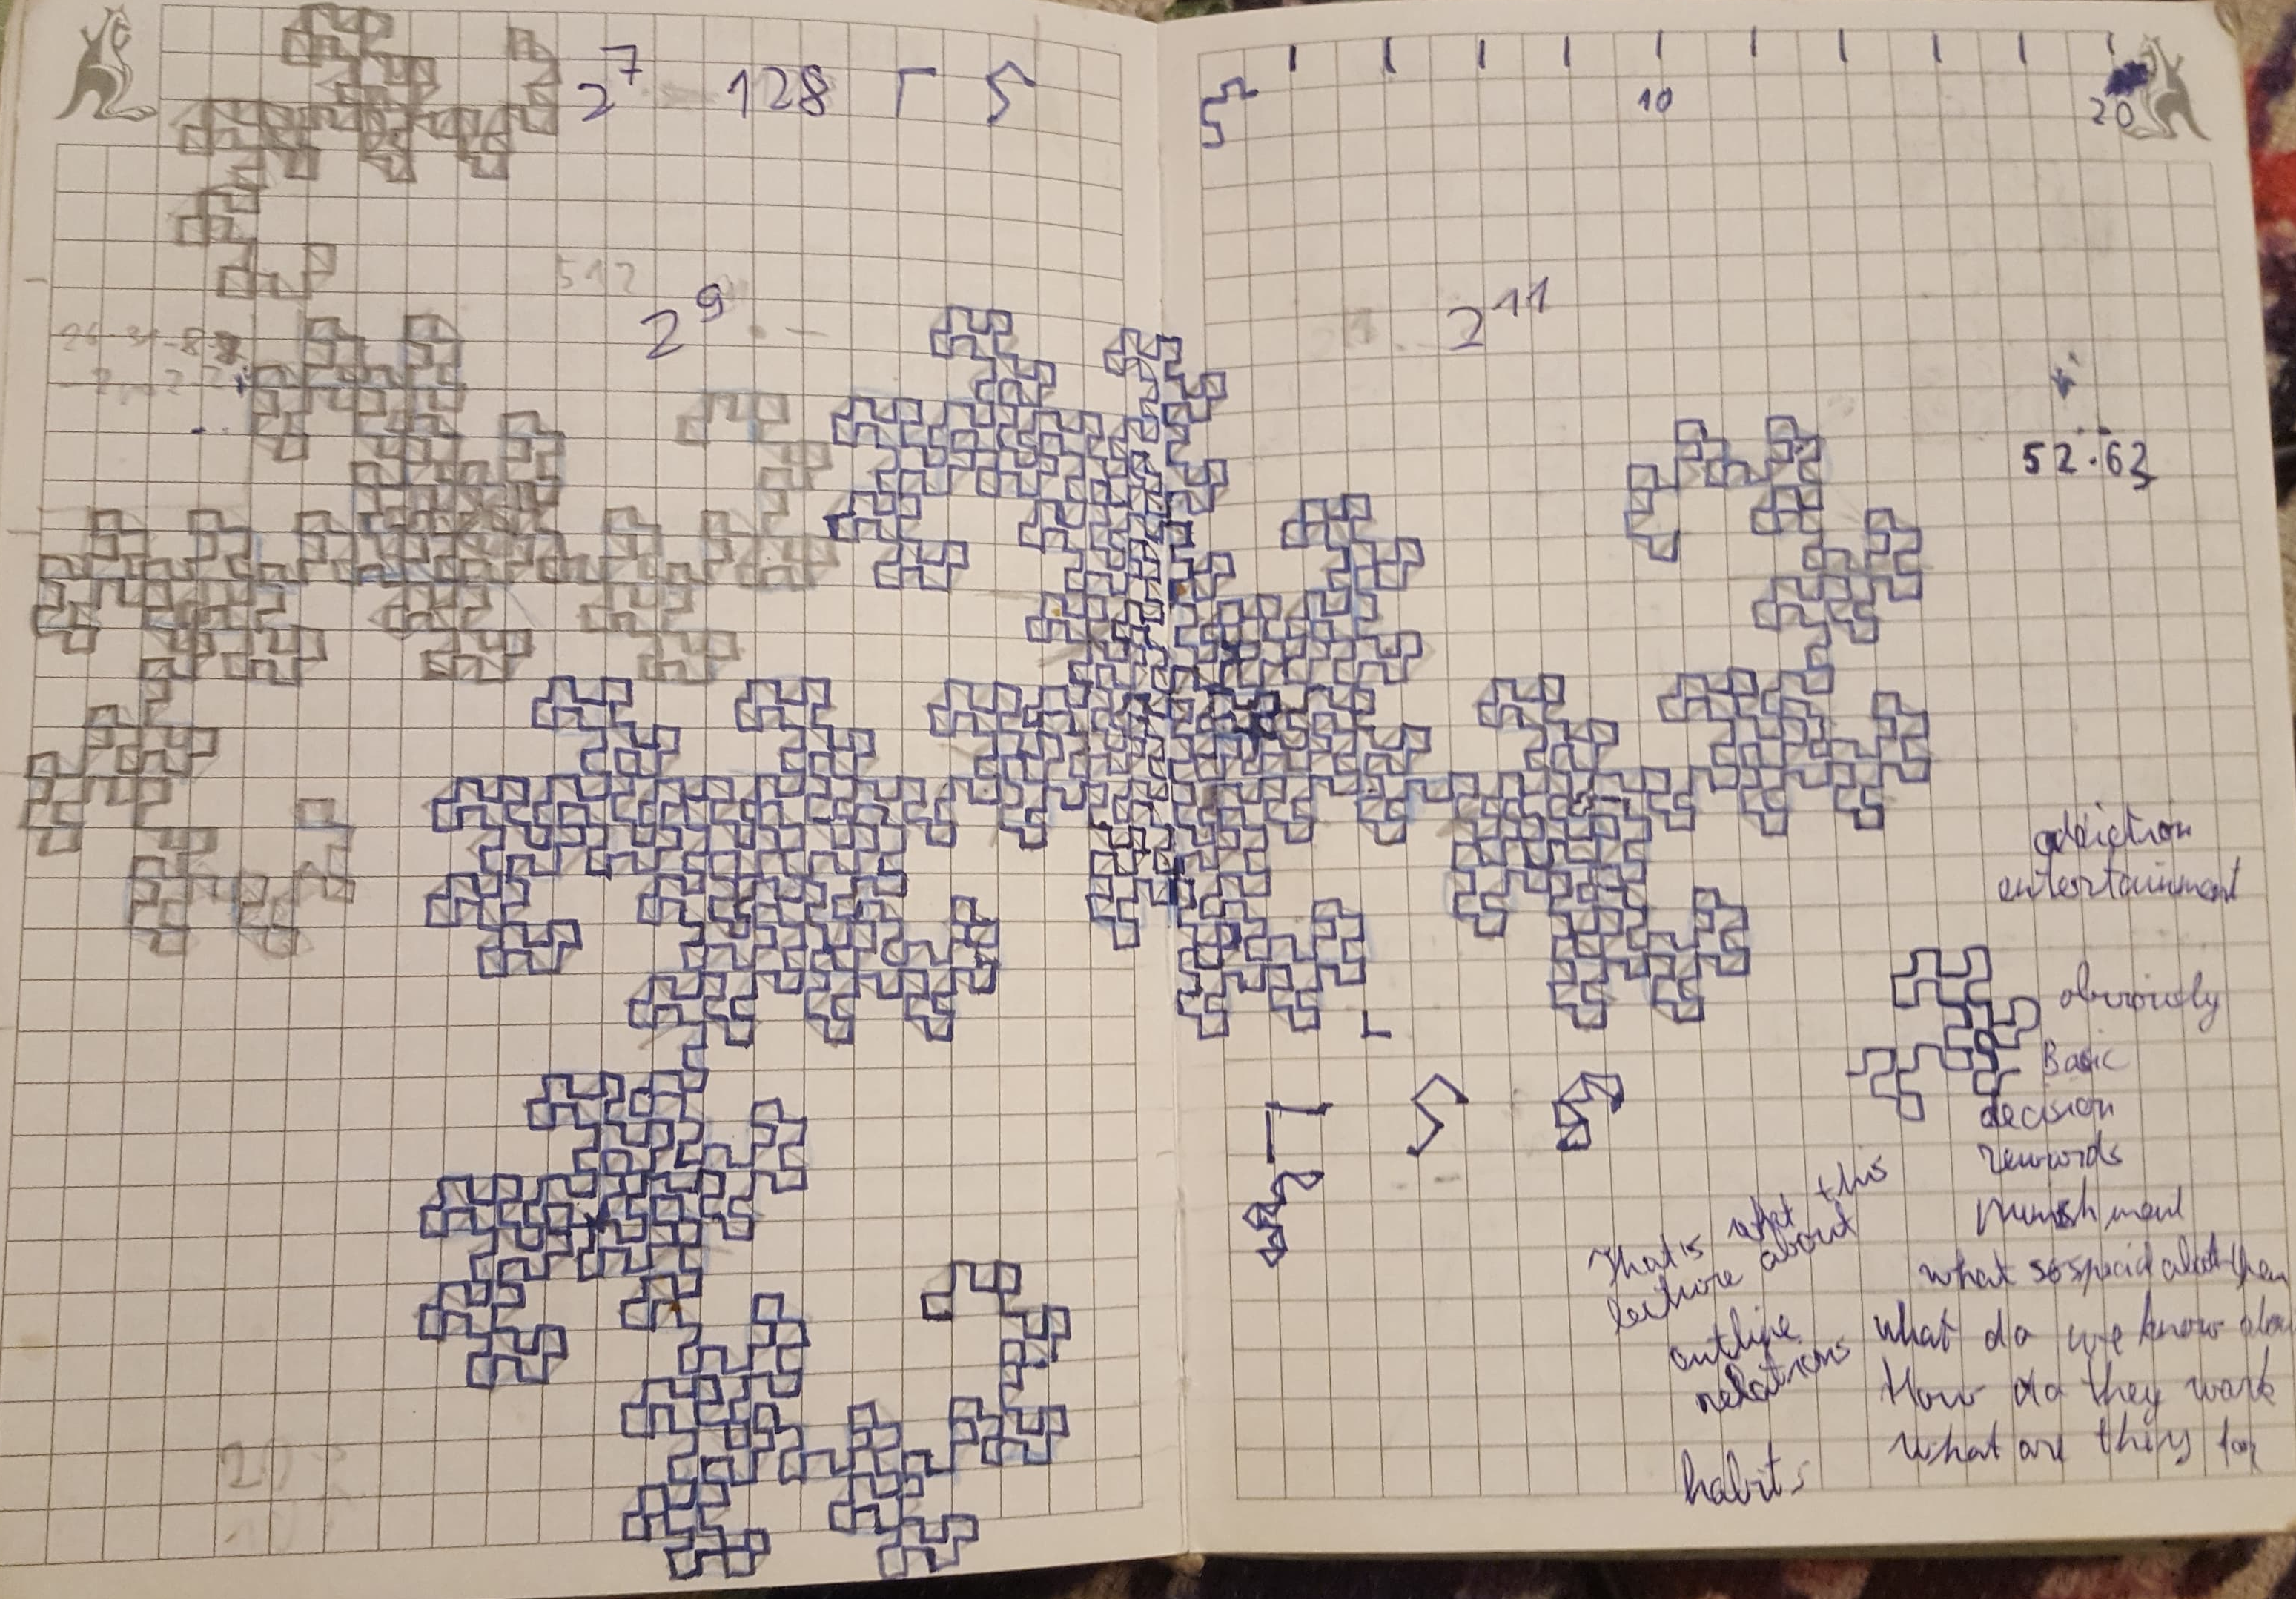
\includegraphics[width=0.7\textwidth]{dragons.png}

Ši kreivė yra vadinama \goto{https://en.wikipedia.org/wiki/Dragon_curve}{Drakono kreive}. Aš ją paišydavau kiekvieną fragmentą ,,\_'' keidamas į fragmentą ,,$/\backslash$''. Po to gautą brėžinį ištrindavau ir vėl perpaišydavau detalesnį brėžinį toje pačioje vietoje. Tad iš pradžių būdavo tik vienas brūkšnys, po to 2, 4, 8, 16 ir t.t. - kaskart po dvigubai daugiau.Vikipedijos \goto{https://en.wikipedia.org/wiki/Dragon_curve}{nuorodoje} kreivę konstruoja kitokiu būdu, bet rezultatas tas pats.

\subsection*{Daugianarių daugyba ir kaip greitai dauginti}

\say{Aš}. Iš to, ką aptarėme, jau pasimatė labai daug apie įvairių fraktalų gavimo būdus. Vis dėlto mūsų pamoka prasidėjo nuo aiškinimosi, kas yra \say{Malderbroto aibė}. Skaitydami apibrėžimą supratome, kas yra aibė \textit{aibė}, bet nesupratome, kas yra kompleksiniai skaičiai, funkcijos, divergavimas ir kas tie keisti užrašai $0,f_{c}(0), f_{c}(f_{c}(0))$. Ir nors mokykloje nekalba apie tokius įdomius dalykus, kaip kompleksiniai skaičiai ir jų veiksmai, aš esu pasiruošęs papasakoti apie juos esminius dalykus. Bet tam mums reikės paskubomis susipažinti su daugianarių daugyba. Tad pradėkime. Įsivaizduokime dvi atkarpas. Tegu viena jų yra sudaryta iš ruožų $a$ ir $b$, o kita iš ruožų $c$ ir $d$. Tuomet kyla klausimas: kam lygus stačiakampio, kurio gretimos kraštinės yra tokios atkarpos, plotas? Sprendimą galima pailiustruoti:

\begin{tabular}{c||c|c}
 & a & b \\ \hline \hline
 c & ac & bc\\ \hline 
 d & ad &bd
\end{tabular}

Vadinasi, plotą galima užrašyti dvejopai: arba kaip skaičių $a+b$ ir $c+d$ sandaugą $(a+b)(c+d)$ arba kaip atskirų sandaugų sumą $ac+bc+ad+bd$. Toks būdas leidžia greitai apskaičiuoti reiškinius, kuriuos vengia duoti dauginti mūsų mokyklose, nes dauginimas būtų per sudėtingas. Tačiau aš tokį vieną veiksmą pademonstruosiu. Tarkime, kad mums reikia skaičių $a+b+c$ padauginti iš savęs. Tuomet mano lentelė bus tokia:

\begin{tabular}{c||c|c|c}
 & a & b & c\\ \hline \hline
 a & $a^2$ & ab & ac\\ \hline 
 b & ab & $b^2$ & bc\\ \hline
 c & ac & bc & $c^2$
\end{tabular}

Matome, kad lentelėje nariai $ab$, $bc$ ir $ac$ pasikartoja po dusyk. Todėl turime: $$(a+b+c)\cdot (a+b+c) = a^2+b^2+c^2+2ab+2bc+2ac.$$ Dalį iš tokių rezultatų vadina \goto{https://www.ematematikas.lt/forumas/greitosios-daugybos-formules-t10771.html}{greitosios daugybos formulėmis} ir moko jas 8 klasėje. Tau duosiu pabandyti sudauginti reiškinius $(a+b)(a-b)$

\say{Simonas}. \textit{Daro lentelę. Darydamas įvelia klaidų, bet žino, kaip jas ištaisyti. Prasitaria, kad mokykloje neigiamų skaičių nemoko, bet jis turėjo juos praeitoje mokykloje ir žino, kad $3\times (-5) = -15$. Todėl žino ir, kad $a\times(-b)=-ab$}.

Simono sprendimas:

$\bcancel{\cancel{\begin{array}{c||c|c}
 & a & -b \\ \hline \hline
 a & a^2 & \dots \\ \hline 
 b & ba^2 & -ab
\end{array}}}\phantom{xxx} \begin{array}{c||c|c}
 & a & -b \\ \hline \hline
 a & a^2 & -ab\\ \hline 
 b & ab & -b^2
\end{array}$

\say{Aš}. Gerai. Nepaisant klaidų galutinis rezultatas visai geras. Be to, kai visus langelius dedame, sumoje $a^2-ab+ab-b^2$ nariai $-ab$ ir $ab$ išsiprastina. Vadinasi, turėsime tokią lygybę:

$$(a-b)(a+b)=a^2-b^2$$

Likusias greitosios daugybos formules palikim kitam kartui, nes jos ne tokios aktualios norint suprasti Mandelbroto aibes. Bet nenorėčiau likti vien papasakojęs apie daugianarių daugybą ir nepapasakojęs apie patį svarbiausią triuką, kur ji gali būti panaudota. Štai uždavinys: reikia sudauginti skaičius $67$ ir $73$. Kaip juos daugintum, Simonai?

\say{Simonas}. Čia kažkur jau bus kažkokia gudrybė, bet aš nežinau kur. Aš matyt dauginčiau $67$ iš $7$ ir dėčiau su $67$, padaugintu iš $3$ (vieną užrašytą po kitu, kaip reikia).

\say{Aš}. Taip, bus gudrybė. Šį uždavinį aš daryčiau mintinai ir užtrukčiau ne daugiau kaip dvi sekundes. Štai mano sprendimas:

$67\times 73 = (70-3)\times (70 + 3) = 70^2 - 3^2 = 4900 - 9 = 4891$

Tiesa, skaičių 70 aš randu imdamas vidurį tarp 67 ir 73. Tuomet ir 67 ir 73 skiriasi nuo 70 po tris.

\say{Simonas}. Oho...

\say{Aš}. O dabar tu pamėgink. Tegu veiksmas bus $37 \times 53$. 

\say{Simonas}. Nežinau, kaip čia...

\say{Aš}. Na, o koks bus vidurys?

\say{Simonas}. 40. Ai ne, juk čia 53. Tada 45.

\say{Aš}. Gerai, tęsk. 

\say{Simonas}. Gavau 1225. 

\say{Aš}. Oj, tikrai neteisingai. Parodyk, kaip skaičiavai?

\say{Simonas}. $45\times 45 = 2025$, tada... Oi, kokia klaida. Aš atėmiau 800, o reikėjo atimti 64...

\say{Aš}. Na va, mes norim išsiaiškinti apie Malderbroto aibes, o net paprasti veiksmai nesigauna. Šio uždavinio sprendimas toks:

 $37 \times 53 = (45 - 8)(45+8)=45^2-8^2=2025-64=1961$
 
 Visgi labai gerai, kad supranti idėjas. Mes atradom labai įdomų dalyką: dviženklių skaičių daugyba greičiausiai eitųsi daug lengviau, jei ne tik mokėtume greit skaičiuoti vidurius su skirtumais,  bet būtume įsiminę visus dviženklių skaičių kvadratus. 
 
 \subsection*{Nuokrypis į matematikos istoriją}
 \say{Aš}. Tai, ką mes iki dabar darėme, buvo susipažinimas su moderniąja, t.y. pačia naujausia 20 amžiaus matematika. Aš išskirčiau tris tarpsnius, kurlink judėjo matematika:
 \begin{itemize}
 \item Antikos laikais rasti tam tikrą ilgį reiškė atlikti geometrinę konstrukciją (vien linijos ir skriestuvo pagalba), iš kurios matyti, kaip tą ilgį gauti. Tais laikais geometrai buvo labai stiprūs, o pati geometrija vadinama euklidine. Tai reiškia, kad mažai kalbama apie kitokius dalykus, nei kampai, atkarpos, tiesės, taškai, apskritimai, pusiaukraštinės, pusiaukampinės, daugiakampiai ir pan.
 \item Renesanso laikais matematikos vis didesnę dalį ėmė užimti mokslas apie judėjimą. Kokiu keliu juda patrankos sviedinys? Kaip sukasi planetos apie Saulę? \goto{https://en.wikipedia.org/wiki/Cardioid}{Kaip spindi} šviesa arbatos puodelyje? \goto{https://en.wikipedia.org/wiki/Cycloid}{Kokiu keliu} juda dviračio rato stipinas? \goto{https://en.wikipedia.org/wiki/List_of_curves}{Štai čia} galima rasti daugybę kreivių pavyzdžių.
 \item Naujausiais laikais atsirado dar viena geometrija - fraktalų geometrija. Tokie patys begaliniai atsikartojimai, kuriuos mes nagrinėjom. Tačiau yra kur kas sudėtingiau. Spalvingoji Mandelbroto aibė, kurios artinimą mes stebėjom, buvo gauta panaudojant kompleksinius skaičius ir jų savybes. Kaip ir daugybė kitų įstabių fraktalų
 \end{itemize}
 
 \say{Papildoma informacija}, kurios nepaminėjau per pamoką. Dekarto įvesta koordinačių sistema, kurią mes mokomės mokykloje, buvo genialus įrankis susieti geometrijos ir algebros žinias. Ją pasitelkę 17a. antros pusės matematikai Niutonas ir Leibnicas sugebėjo aprašyti planetų judėjimą ir sukurti naują teoriją apie visatos judėjimą. Skaičiavimo technologijos, kuriomis žmonės remiasi paleisdami palydovus skristi virš Žemės ir kuriomis suplanavo Žmonių išsilaipinimą Mėnulyje ir net paleido aparatą, išskridusį už Saulės sistemos ribų, - visa tai Niutono ir Leibnico laikų matematikos palikimas.
 
 Tačiau besibaigiant 17 - ajam amžiui kompleksinių skaičių veiksmai vis dar buvo paslaptimi. Niutonas juos atmetė kaip neturinčius jokios geometrinės ir fizikinės prasmės. Leibnicas skaičių $\sqrt{-1}$ apibūdino kaip idealaus pasaulio pranašą, kuris yra tarsi amfibija tarp būties ir nebūties. Ir nors ankstyvojo renesanso intelektualas John Wallis siūlė į skaičių $x+y\sqrt{-1}$ žvelgti kaip į tašką koordinačių plokštumoje, kuris turi koordinates $(x; y)$, ši idėja nesusilaukė dėmesio. Vietoj to, algebrinius metodus, kurie galiojo su teigiamais skaičiais, ėmė taikyti ir neigiamiems skaičiams ir taip gaudavosi lygčių sprendimo rezultatai, neturintys jokios prasmės. 
 
Neaiškumus prasklaidė matematikas Oileris. Jis įvedė žymėjimą $i=\sqrt{-1}$ ir priprato visur kompleksinių skaičių veiksmuose pamatęs reiškinį $i^2$ jį pakeisti skaičiumi -1, o tokius skaičius kaip $\sqrt{-3}$ žymėti $i\sqrt{3}$. Oileris išvedė būdus, kaip pavaizduoti kompleksinių skaičių sudėtį ir daugybą koordinačių plokštumoje. Dabar kompleksiniai skaičiai jau įgavo visai kitą prasmę. Galima sakyti, geometrinės interpretacijos atradimas užtruko visą amžių arba daugiau.
 
 \say{Simonas}. Kažin, kai taip viskas vystosi, kas gi dėsis dar toliau?
 
 \say{Aš}. Aš pats tai nemanau, kad kažkas stipriai kitokio dėsis. Praeitą pamoką buvau užsiminęs, kad topologiją sujungus su vaizdo atpažinimo algoritmais buvo mokslinkų pastebėta, kad tolimiausiuose visatos kampuose galaktikos jungiasi kažkuo, kas panašu į gijomis susipynusius debesėlius. Tačiau ne visai tą galima vadinti matematika. Jau greičiau tai galima vadinti matematikos taikymais. O patys matematikai tik gerina vaizdo atpažinimo algoritmus, įrodo vis naujas teoremas topologijoje. Galbūt matematinių žinių poreikis tiriant kosmose ir paspartints matematinius atradimus tam tikrose srityse. Tačiau yra vienas didelis skirtumas tarp dabartinės ir ankstesnės matematikos. Dabar mokslininkai dirba siaurose srityse. Tokiose kaip Kardioidės kreivės praplėtimas $n$ - matėje erdvėje. Tačiau dabartinės matematikos žinios yra neaprėpiamos vieno žmogaus protui taip, kaip per antiką arba per renesansą. Paskutinis genijus, kuris buvo pajėgus suprasti visą matematiką, mirė prieš 100 - 150 metų (neatsimenu vardo, bet jį galima rasti knygoje \textit{V. Stakėnas. Matematikos istorijos skiautiniai}). Dabartinėje matematikoje gamtoje vykstantys judėjimai didžiąja dalimi jau senai ištyrinėti, taigi jų teorija neturėtų stipriai keistis.
 
 \say{Simonas}. O tai ką nagrinėja matematikos mokslininkai dabar?
 
 \say{Aš}. Imkime štai pavyzdžiui vieną mūsų šalyje sėkmingiausių tavo tėvų amžiaus matematiką Giedrių Alkauską. Jį aš pažįstu kaip poetą, kompozitorių ir matematikos mokslininką. Kaip jis sako - aš pusantrų metų skiriu muzikai, o po to pusantrų matematikai. \goto{https://www.facebook.com/giedrius.alkauskas/posts/1327817344001999}{Štai čia} nuėję iš pirmų lūpų išgirstume jo pristatymą apie pačius naujausius jo mokslinius darbus. Ar ką nors pavyko suprasti?
 
 \say{Simonas}. Ne.
 
 \say{Aš}. Man beveik irgi ne.

\subsection*{Kompleksinių skaičių sudėjimai ir dauginimai}
\noindent\begin{minipage}[b]{0.69\textwidth}
\say{Aš}. Prieš pradedant kalbėti apie kompleksinius skaičius reiktų mažų mažiausiai žinoti, kaip bet kuris taškas gali būti aprašytas skaičiais. Mano kompiuteryje matome įjungtą programą \goto{https://www.geogebra.org/download}{Geogebra Classic 6}. Tai labai populiari programa, kurią naudoja visas pasaulis. Pavyzdžiui šios programos naudojimas yra įtrauktas į prancūzų moksleivių matematikos programą. Dabar savo kompiuteryje aš pažymėsiu vieną tašką. Ar galėtum pasakyti jo ,,skaičius''?

\say{Simonas}. Taip, tai būtų koordinatės (2; 3).

\say{Aš}. Žinoma, teisingai. Kiekvienam taškui aprašyti reikia dviejų skaičių, vadinamų jo koordinatėmis, ir ne kitaip. O dabar pažymėsiu keletą kitų taškų. Kokios yra jų koordinatės?

\say{Simonas}. (1; 5), (-2; 2) ir (1; 3).

\say{Aš}. Viskas būtų gerai, tik taško C koordinatę pasakei visai ne tokią.

\say{Simonas}. Aaa... Tai turi būti (1; -3).

\say{Aš}. Na matai. Tai ir su paprasta koordinačių sistema trūksta patirties. Ką ir bekalbėti apie kompleksinius skaičius, kurių mokykloje nebus. Tačiau laiko mes daug neturim ir reikia pagaliau atsakyti į klausimą, kas ta Malderbroto aibė, tad iš karto eisim prie kompleksinių skaičių. Tik ateičiai tau, Simonai, reiktų nepamiršti, kad ir paprastoje koordinačių sistemoje,\end{minipage}
\begin{minipage}[b]{0.3\textwidth}
\includegraphics[width=\textwidth]{taskai.png}
\end{minipage}
kurią eina kaip tik šeštoje klasėje, tu dar ne visai gaudaisi. Tu jau minėjai, kad šį tą žinai apie neigiamus skaičius, nors mokykloje juos eisite tik kitoje klasėje. Pavyzdžiui, kam lygu $-3 \times (-5)$? 

\say{Simonas}. Aš atsimenu, kad 15.

\say{Aš}. Taip, teisingai. Sudauginus du neigiamus skaičius visuomet gausime teigiamą. Tačiau renesanso pradžioje neigiami skaičiai buvo kažkas, ką matematikai vengė naudoti. Labiausiai juos erzino, kad negalime traukti iš jų šaknies. Pavyzdžiui, juk galima ištraukti iš 9 šaknį?

\say{Simonas}. Aš galiu. Tai bus 3.

\say{Aš}. O kokia būtų šaknis iš $-9$?

\say{Simonas}. Nežinau. Galvoju, kad tai nesąmonė. Iš tikrųjų, 3 negali būti. Bet negali būti ir $-3$, nes jį padauginę su savimi turėsime 9.

\begin{minipage}[b]{0.69\textwidth}
\say{Aš}. Labai geros mintys. Iš tiesų, šaknis iš $-9$ negali būti traukiama. Nesigauna joks skaičius, kurio sandauga su savimi būtų $-9$. Tačiau, jei matematikai nebūtų apsimetę, kad toks skaičius \textit{yra}, tai matematika visai nebūtų pasistūmusi į priekį. Taigi, jie paėmė ir pažymėjo skaičių $\sqrt{-1}$ simboliu $i$ (\textit{imaginary} - įsivaizduojamas). Paaiškėjo, kad visos dauginimo ir sudėties taisyklės, kurias mes šiandien šiek tiek pasimokėme su daugianariais, tokiems skaičiams irgi tinka. Pavyzdžiui, paimkime skaičių $2+3i$. Jame yra ,,kažkiek'' realiosios dalies ir ,,kažkie''' įsivaizduojamos. Realiosios dalies dydis yra 2, o įsivaizduojamos, kuri pasako, kiek skaičiuje yra šaknų iš $-1$, dydis yra 3. Pavyzdžiui imkime ir sudėkime du kompleksinius skaičius: $2+3i$ ir $1+2i$. Dabar galime pasižiūrėti, kaip jie sudedami koordinačių plokštumoje. Ar galėtum joje pažymėti taškus $(2;3)$ ir $(1;2)$. 

\say{Simonas}. Taip, štai jie.

\say{Aš}. Teisingai. Dabar aš pasiimsiu tašką $A$ ir paslinksiu jį taip, kaip yra pasislinkęs taškas $B$ nuo 0. Mano brėžinys atrodys štai taip. Ar supranti, kas čia įvyko? 

\say{Simonas}. Tiesą sakant, nelabai.
\end{minipage}
\begin{minipage}[b]{0.3\textwidth}
\includegraphics[width=\textwidth]{sudetis.png}
\end{minipage}

\say{Aš}. Na, nieko keisto. Šitas dalykas nėra pats sudėtingiausias, tačiau jį vis tiek mokina tik 11 klasėje. Tiesa, tema, kur reikia slankioti taškus, vadinasi \textit{vektoriai}. Tačiau vienuoliktokai ją taip greit išeina, kad dažnai ir nespėja suprasti, kas tie vektoriai. Manau, jog su kompleksinių skaičių sudėtimi šiandien daug mokytis neverta. Tau užteks žinoti, kad kompleksiniai skaičiai gali būti vaizduojami kaip taškai koordinačių plokštumoje, ir kad juos sudėję mes gauname kitą skaičių, kurio vietą plokštumoje taip pat galima gauti ir geometriškai. Šiuo atveju matome, kad gaunasi gražus lygiagretainis. O dabar panagrinėkime kompleksinių skaičių daugybą. Tuoj duosiu tau užduotėlę. Ar galėtum sudauginti išraišką $1+i$ su savimi taip, kaip mes mokėmės su lentelėmis?

\say{Simonas}. (Manęs padedamas bando):

$\begin{array}{c||c|c}
 & 1 & i \\ \hline \hline
1 & 1 & i\\ \hline 
 i & i & ?
\end{array}$

Nesuprantu, kaip toliau daryti.

\say{Aš}. Norint suprasti, kam lygu $i \times i$, reiktų labiau pamąstyti apie tai, kaip mes suprantame, kas yra šaknis iš skaičiaus. Kaip tu supranti šaknį?

\say{Simonas}. Tai yra tai, ką reikia padauginti iš savęs, kad gautume pošaknį.

\say{Aš}. Teisingai. O ką reikia padauginti iš savęs, kad gautume $-1$? 

\say{Simonas}. Bet juk tokio skaičiaus nėra. Jei dauginame neigiamą iš neigiamo, gausime teigiamą. Su teigiamais - tuo labiau. 

\say{Aš}. Bet mes juk tik ką kalbėjome, kad skaičius $i=\sqrt{-1}$, yra būtent tai, ką reikia padauginti iš savęs, kad gautume $-1$.  Vadinasi $i\times i = -1$. Ir nepaisant to, kad skaičiaus $i$ tikrovėje nėra, o matematikai turėjo apsimesti, kad jis yra, mes su juo atliekame veiksmus. Baigiame pildyti lentelę:

$\begin{array}{c||c|c}
 & 1 & i \\ \hline \hline
1 & 1 & i\\ \hline 
 i & i & -1
\end{array}$

Į ką susideda visi langeliai?

\say{Simonas}. Na, 1 ir 1 atsiima, tai lieka $i$ ir $i$. Tada gaunasi $2i$. 

\say{Aš}. Taip, visi langeliai susideda į $2i$. Gaunasi netikėtas rezultatas: $(1+i)^2=2i$. Tolimesnę pamoką kompleksinių skaičių nedauginsime, nes jie juk neįeina į mokyklinę programą. Paliksiu šį darbą kompiuteriui. Tik prieš tai man reikės šiek tiek laiko paprogramuoti, o tu galėsi pamatyti, kaip greitai šiais laikais galima atlikti matematinius skaičiavimus naudojant kompiuterį.

\say{(Po 3 minučių programavimo.)}

\begin{minted}{python}
import sympy as sp
from IPython.display import display
sp.init_printing()
z, c1, c2 = sp.symbols("z c1, c2", real=True)  
c1, c2 = 1, 1
c = c1+sp.I*c2
z= c
print(r'$\begin{array}{|c|c|c|}\hline')
for i in range(11):
    #print('&'.join([str(i+1),sp.latex(z),sp.latex(sp.expand_complex(z))])+r'\\ \hline')
    display(sp.expand_complex(z))
    z=z*c
print(r'\end{array}$')
\end{minted}

Savo programoje aš skaičių $1+i$ dauginu iš savęs 10 kartų. 
\newline
\newline
\begin{minipage}[b]{0.3\textwidth}
Programa išmeta tokį rezultatą:

$\begin{array}{|c|c|c|}\hline
\text{Žingsnis} & \text{Veiksmas} & \text{Rezultatas} \\ \hline \hline
1&1 + i&1 + i\\ \hline
2&\left(1 + i\right)^{2}&2 i\\ \hline
3&\left(1 + i\right)^{3}&-2 + 2 i\\ \hline
4&\left(1 + i\right)^{4}&-4\\ \hline
5&\left(1 + i\right)^{5}&-4 - 4 i\\ \hline
6&\left(1 + i\right)^{6}&- 8 i\\ \hline
7&\left(1 + i\right)^{7}&8 - 8 i\\ \hline
8&\left(1 + i\right)^{8}&16\\ \hline
9&\left(1 + i\right)^{9}&16 + 16 i\\ \hline
10&\left(1 + i\right)^{10}&32 i\\ \hline
\end{array}$
\end{minipage}
\hspace{\fill}
\begin{minipage}[b]{0.6\textwidth}
Šalia parašysiu tuos skaičius atitinkančių taškų koordinates:

$\begin{array}{|l|}\hline
\text{Koordinatė}\\ \hline \hline
(1;1)\phantom{\left(\right)^2}\\ \hline
(0;2)\phantom{\left(\right)^2}\\ \hline
(-2;2)\phantom{\left(\right)^2}\\ \hline
(-4;0)\phantom{\left(\right)^2}\\ \hline
(-4;-4)\phantom{\left(\right)^2}\\ \hline
(0;-8)\phantom{\left(\right)^2}\\ \hline
(8;-8)\phantom{\left(\right)^2}\\ \hline
(16;0)\phantom{\left(\right)^2}\\ \hline
(16;16)\phantom{\left(\right)^2}\\ \hline
(0;32)\phantom{\left(\right)^2}\\ \hline
\end{array}$
\end{minipage}

Simonai, ar galėtum gautus taškus pavaizduoti koordinačių plokštumoje kompiuteryje?

\say{Simonas}. Galima pelę? \textit{(Vaizduoja taškus)}... Štai taip \textit{(Paveikslėlyje)} 

\say{Aš}. (Lyg ir) vienas taškas iš pradžių pažymėti nesigavo, bet visi kiti gerai.
\subsection*{Paskutiniai štrichai suvokiant įstabųjį fraktalą}
\begin{minipage}[b]{0.68\textwidth}
\say{Simonas}. Klausykite, mums tuoj bus likęs tik pusvalandis laiko. Gal bus galima jau eiti prie erdvinių kūnų, nes aš noriu dar iš jų pasiruošti.

\say{Aš}. Gerai, būtinai. Iš tikrųjų, mums jau liko visai nedaug. Tokį didelį darbą padarėm, tad gaila būtų neužbaigti. Kaip manai, kaip koordinačių plokštumoje būtų išsidėstę grafiko taškai, jei tęstume toliau?

\say{Simonas}. Manau, jog eis į begalybę ir gausis spiralė.

\say{Aš}. Taip, teisingai. Artėjimas į begalybę net gi turi savo pavadinimą: \textit{divergavimas}. Tai štai, ką Vikipedija turėjo mintyje sakydama, kad sekos nariai artėja į begalybę. Aš tuojau šiek tiek pagražinsiu savo brėžinį: 

\includegraphics[width=0.8\textwidth]{kriaukle.png}
\end{minipage}
\hspace{\fill}
\begin{minipage}[b]{0.3\textwidth}

\say{Štai čia Simonas vaizduoja taškus:}

\includegraphics[width=\textwidth]{sraige.png}
\end{minipage}

\say{Aš}. Tai štai kokios galios slypi kompleksiniuose skaičiuose. Jų daugyboje atsispindi fraktalai! Kaip tai vyksta? 

Kompleksiniai skaičiai turi nuostabią savybę: kai juos daugini, jų pasisukimai nuo $x$ koordinatės susideda, o atstumai nuo koordinačių pradžios susidaugina. Pavyzdžiui skaičius $1+i$ turi pasisukimą, lygų 45 laipsniams ir ilgį, lygų $\sqrt{2}$. Jei jį padauginsime iš savęs, darsyk prisidės toks pats kampas, o nuotolis nuo koordinačių pradžios taško susidaugins su $\sqrt{2}$ ir gausis ilgis, lygus 2. Todėl į skaičių $(1+i)^2$ atitinkantį tašką nukreipta atkarpa bus pasisukusi 90 laipsnių. O jei $(1+i)^2$ padaugintume dar iš $1+i$, tai pamatytume, kad naujoji atkarpa jau yra pasisukusi 135 laipsniais nuo $x$, o jos ilgis yra jau $2\sqrt{2}$.

Tačiau, deja, ne visus kompleksinius skaičius vis dauginant su savimi turėsime artėjimą į begalybę. Kartais taip dauginant kompleksinius skaičius jau greičiau važiuosime link tam tikro taško, negu, kad į begalybę. 

Na, o dabar jau įmanoma paaiškinti, ir kas ta Malderbroto aibė. Tai yra aibė, sudaryta iš tokių kompleksinių skaičių, kuomet pakartotinai atliekant tam tikrą veiksmą, rezultatai artės link tam tikro skaičiaus, bet ne į begalybę. Šie skaičiai atitinka koordinačių plokštumos taškus. Jie yra išsidėstę taip įdomiai, kaip ligi praeito amžiaus galo dar niekas nebuvo matę. Paveikslėlyje matome juodą sritį. Ji sudaryta, iš juodų taškų. Šie juodi taškai atitinka skaičius, su kuriais pakartotinai atliekant tą pačią operaciją, nauji rezultatai artės į tam tikrą sritį, kuri nėra ties begalybe. Tuo tarpu atliekant tą operaciją su užribyje likusiais taškais, gausime rezultatus, kurie bus vis artimesni begalybei, kaip ir toje kriauklėje, kurią nagrinėjome. Na, o jei dar pridėsime spalvas ir jas parinksime pagal tai, kokiu greičiu skaičiai artėja į begalybę, tai ir gausime įstabųjį mirguliuojantį Mandelbroto fraktalą.

\subsection*{Moralas}

Informacijos internete yra labai daug, bet ar tikrai aišku, kaip ja naudotis?

\begin{itemize}
\item Ar aš tikrai suprantu tai, apie ką skaitau? Kas ta \textit{Malderbroto} aibė? Kiek kartų ji priartinama?
\item Ar aš tikrai suprantu kiekvieną žodį, einantį į tiriamo objekto apibrėžimą. Ką reiškia apibrėžime naudojamos sąvokos: \textit{complex numbers}, \textit{functions}, \textit{diverge}, \textit{iterated}, \textit{bounded}?
\item Ar teiginiai tikrai teisingi? Ar aibės padidinimas $10^{198}$ kartų tikrai yra pasaulio rekordas?
\item Kur ieškotume reikiamos informacijos? \goto{https://www.google.com/}{Google}, \goto{https://www.youtube.com/watch?v=X_tYrnv_o6A}{Youtube}, \goto{https://lt.wikipedia.org/wiki/Fizikinis_dydis}{lietuviška Vikipedija}, \goto{https://en.wikipedia.org/wiki/Quantity}{angliška Vikipedija}, \goto{https://www.quora.com/What-is-the-Mandelbrot-set-1}{Quora}, \goto{https://www.wolframalpha.com/input/?i=(1\%2Bi)\%5E8}{Wolfram}
\end{itemize}

\subsection*{Detalės, likusios užkulisiuose, bet nemažiau svarbios}

Operacija, kurią pakatotinai atlieka, Malderbroto aibėje yra kėlimas kvadratu ir pasirinkto skaičiaus $c$ pridėjimas. Pavyzdžiui, jei $c=i$, tai gaunasi tokia seka:
 
$\tiny\begin{array}{|c|c|c|}\hline \begin{array}{c}\text{Sekos}\\ \text{narys}\end{array} & \text{Nesuprastinta skaičiaus išraiška} & \text{Suprastinta išraiška} \\ \hline \hline
0&0&0\\ \hline
1&i&i\\ \hline
2&-1 + i&-1 + i\\ \hline
3&\left(-1 + i\right)^{2} + i&- i\\ \hline
4&\left(\left(-1 + i\right)^{2} + i\right)^{2} + i&-1 + i\\ \hline
5&\left(\left(\left(-1 + i\right)^{2} + i\right)^{2} + i\right)^{2} + i&- i\\ \hline
6&\left(\left(\left(\left(-1 + i\right)^{2} + i\right)^{2} + i\right)^{2} + i\right)^{2} + i&-1 + i\\ \hline
7&\left(\left(\left(\left(\left(-1 + i\right)^{2} + i\right)^{2} + i\right)^{2} + i\right)^{2} + i\right)^{2} + i&- i\\ \hline
8&\left(\left(\left(\left(\left(\left(-1 + i\right)^{2} + i\right)^{2} + i\right)^{2} + i\right)^{2} + i\right)^{2} + i\right)^{2} + i&-1 + i\\ \hline
9&\left(\left(\left(\left(\left(\left(\left(-1 + i\right)^{2} + i\right)^{2} + i\right)^{2} + i\right)^{2} + i\right)^{2} + i\right)^{2} + i\right)^{2} + i&- i\\ \hline
10&\left(\left(\left(\left(\left(\left(\left(\left(-1 + i\right)^{2} + i\right)^{2} + i\right)^{2} + i\right)^{2} + i\right)^{2} + i\right)^{2} + i\right)^{2} + i\right)^{2} + i&-1 + i\\ \hline
\end{array}$

Kadangi nėra artėjimo į begalybę, tai skaičius $c = i$ priklauso Malderbroto aibei.

Geogebros puslapyje yra patalpinta interaktyvi žingsnių Malderbroto aibėje \goto{https://www.geogebra.org/m/Npd3kBKn}{vizualizacija}. Ant fraktalo galima užvesti tašką, kuris atitinka skaičių $c$. Tuomet paveikslėlyje bus pailiustruotas taškų, gautų sekos $0$, $c$, $c^2+c...$ kiekvieną narį pakeliant kvadratu ir pridedant $c$, rinkinys. Malderbroto aibėje bus stebimas sekos narių artėjimas į vieną tašką, o už jos ribų - vis platesnis išsiskirstymas.

\subsection*{UŽDUOTYS}
Nors pateikiamus pratimus galima išspręsti remiantis šia medžiaga, tačiau į pateikiamus klausimus atsakymų reiktų ieškoti internete. Atsakymų spėlioti nereikėtų, o vietoj to reikėtų įgusti susirasti reikiamą informaciją internete per kuo trumpesnį laiką.
\begin{enumerate}
\begin{minipage}[b]{0.65\textwidth}
\item Kas vadinama fraktalu?
\item Kada buvo atrasta Malderbroto aibė?
\begin{framed}
Kaip pasileisti python?
\begin{itemize}
\item Reikės atsisiųsti jį \goto{https://www.python.org/downloads/}{iš čia}
\item Reikės aplinkos su kuria dirbsime. Patartina naudoti \goto{https://www.spyder-ide.org/}{Spyder}
\end{itemize}
\end{framed}
\item Pabandykite susiinstaliuoti Python savo kompiuteryje ir paleisti šias eilutes:
\begin{minted}{python}
from time import*
t=time(); [i**2 for i in range(10000000)]; print(time()-t)
\end{minted}
Programa naudoja \mintinline{python}{time} modulį, kad apskaičiuotų savo veikimo laiką. Pačioje programoje yra keliami kvadratu skaičiai nuo 0 iki 10000000 milijonų. Kiek laiko kvadratu yra keliamas vienas skaičius? Kaip pasikeis situacija, jei skaičių kelsime kubu?
\begin{framed}
\goto{https://www.wahl.org/fe/HTML_version/link/FE3W/c3.htm}{šiame puslapyje} yra apžvelgiami žymiausi fraktalai.
\end{framed}
\item Ar galite pratęsti šią seką?

\includegraphics[width=0.5\textwidth]{dragonsteps.png}

\item  Tęsiant šią seką kaip parodyta yra gaunamas vis tikslesnis Drakono kreivės priartinimas. Kaip pasikeis kreivės ilgis po bet kurių 10 žingsnių?
\end{minipage}
\hspace{\fill}
\begin{minipage}[b]{0.3\textwidth}
\includegraphics[width=\textwidth]{ikoch.png}
\end{minipage}

\item Kokie yra pavaizduotų kreivių ilgiai, jei pirmosios ilgis yra lygus 1? (pav. dešinėje)

\item Ar jums pavyks nupiešti keturmatį kubą? Jį gausite pateiktoje sekoje suradę nežinomą narį:

\includegraphics[width=0.5\textwidth]{hypercube.png}

\begin{framed}
HACK! Jei jums nepavyko sugalvoti atsakymo, dar ne viskas prarasta. Yra būdas, kaip reiktų ieškoti atsakymo internete.
\begin{itemize}
\item Jei naudojate Windows, savo kompiuteryje susiraskite programėlę \say{Snipping Tool} \textit{(Iškarpų įrankis)}.
\item Iš šio failo išsikirpkite sekos paveikslėlį ir išsisaugokite.
\item Google paieškoje paspauskite \say{Images}\textit{(Vaizdai)} ir įkelkite išsaugotą paveiksliuką
\item Jei viskas pavyks, paieška turėtų atrasti panašų paveikslėlį su atsakymu ir nuoroda į tinklalapį, iš kurio paveikslėlis buvo paimtas.
\end{itemize}
\end{framed}

\item Čia pateikiamas Kantoro aibės išėmimų variantas, atliekamas su kubais:

\includegraphics[width=0.16\textwidth]{cantor1.png}
\includegraphics[width=0.16\textwidth]{cantor2.png}
\includegraphics[width=0.16\textwidth]{cantor3.png}
\includegraphics[width=0.16\textwidth]{cantor4.png}
\includegraphics[width=0.16\textwidth]{cantor5.png}
\includegraphics[width=0.16\textwidth]{cantor6.png}

Tarkime, jog pradinio kubo tūris lygus 1. Ar galėtumėte nustatyti kitų kubų tūrius? Link kokio skaičiaus jie artėja?

\item Ankstesnio pratimo iliustracija pateikiama susiradus \goto{https://en.wikipedia.org/wiki/Cantor_set}{angliškos Vikipedijos straipsnį} apie Kantoro aibę. Animaciją galima rasti prie skyrelio ,,Cantor dust''. Tarkime, jog norime sužinoti, kaip toks fraktalas vadinasi. Parodysiu, kaip tokio tinkamo klausimo iškėlimas leidžia atrasti kitų naudingų nuorodų:
\begin{itemize}
\item Animaciją galima rasti prie skyrelio ,,Cantor dust''.
\item Tame pačiame skyrelyje yra pateikiama \goto{https://en.wikipedia.org/wiki/Menger_sponge}{nuoroda} į kitą panašų fraktalą.
\item Iš \goto{https://lt.wikipedia.org/wiki/Fraktalas}{Vikipedijos straipsnio} apie fraktalus arba išsivertę sužinome, kad šis panašus fraktalas vadinamas Mengerio kempine.
\item Ieškome lietuviškų nuorodų apie \href{https://www.google.com/search?q=Mengerio+kempinė\&client=firefox-b-d\&tbm=isch\&source=iu\&ictx=1\&fir=qZ0c-n7YPwP1vM\%253A\%252CqvsowJzBeRJm6M\%252C\_\&vet=1\&usg=AI4\_-kR0ZwupJegAUepmi4xwgf3oq4zEkg\&sa=X\&ved=2ahUKEwj\_i7-ejbjhAhWMo4sKHTDbDSEQ9QEwA3oECCAQCA\#imgrc=Fn0oWIjjZCnT7M:\&vet=1}{\textcolor{blue}{Mengerio kempinę}} ir atrandame \goto{http://www.nso.lt/science/self-quant.htm}{nuorodą}, kurioje kalbama, kaip fraktalai susiję su fizika.
\item Paėję anksčiau matome, kad surastas puslapis gali pasiūlyti ir daugybę kitų lietuviškų ir įdomių straipsnių apie fiziką.
\item Labiausiai mus turėtų dominti straipsnio dalys, kuriose kalba apie fraktalus. Joms surasti naudojame klavišų kombinaciją $CTRL + F$
\item Dažniausiai žodžiuose, prasidedančiuose ,,fraktal'' bus paslėpta nuoroda į kitą interneto adresą. Kokį?
\item Ar galite nuėję į šį adresą matyti įspūdingąsias Mandelbroto fraktalo nuotraukas?
\end{itemize}
Ar remdamiesi šiuo straipsniu galėtumėte atsakyti, kaip fraktalai susiję su fizika? Ar galėtumėte atsakyti ne tik, kada buvo atrasta Malderbroto aibė, bet ir kada žinios apie ją buvo pradėtos populiarinti Lietuvoje?
\begin{framed}
Tolimesnių uždavinių atsakymus padės pasitikrinti \goto{https://www.wolframalpha.com/input/?i=(x-sqrt(2019))(x\%2Bsqrt(2019))}{Wolfram Alpha}
\end{framed}
\item \texttt{Ši užduotis atitinka dabartinės mokyklos 8 klasę, tačiau čia pristatomas jų atlikimo metodas yra daug paprastesnis už mokykloje mokomą kitą metodą. Kompleksiniai skaičiai mokykloje nemokomi, tačiau jų veiksmus galima atlikti remiantis šiuo palengvintu (lentelės) metodu.}

Atlikite šiuos veiksmus remdamiesi lentelėmis:

\begin{tasks}(3)
\task $51 \times 69 = (60 - 9) \times (60 + 9) = ?$
\task $89 \times 91 = ?$
\task $49 \times 49 = (50 -1) \times (50 - 1) = ?$
\task $64 \times 64 = (60 + 4) \times (60 + 4) = ?$
\task $(x-2)\times (x+2) = ?$
\task $(x-\sqrt{3})\times (x+\sqrt{3}) = ?$
\task $(x+2) \times (x+2) = ?$
\task $(x-3) \times (x-3) = ?$
\task $(a+b) \times (a+b) = ?$
\task $(a-b) \times (a-b) = ?$
\task $(a+b) \times (a-b) = ?$
\task $(a+b) \times (a^2-ab+b^2) = ?$
\task $(a-b) \times (a^2+ab+b^2) = ?$
\task $(x-1)\times (x^3+x^2+x+1) = ?$
\task $(x-1)\times (x^7+x^6+x^5+x^4+x^3+x^2+x+1) = ?$
\task $(x^2-2x+2)\times (x^2+2x+2)=?$
\task *$(a+b+c)\times (a+b+c)=?$
\task *$(a+b+c)\times (a^2+b^2+c^2-ab-bc-ca)=?$
\task *$(1+x+x^2+x^3)\times (1+x+x^2+x^3)=?$
\task *$(a-b)(b-c)(c-a)=?$
\task $(1+2i)\times (2+3i)=?$
\task $(1+2i)\times (1-2i)=?$
\task $(x+i)(x-i)=?$
\task $(x+x^2+x^3+x^4+x^5+x^6)\times (x+x^2+x^3+x^4+x^5+x^6)=?$
\end{tasks}
\item \textcolor{green}{\say{IDĖJA KITAM PROJEKTUI.}} \goto{https://www.youtube.com/watch?v=M4vqr3_ROIk}{Šiame video} publiką stulbina žmogus, galintis per minutę sudauginti du penkiaženklius skaičius. Ar galėtumėte apibūdinti bent keletą jo naudojamų metodų? Ar šis veikėjas galėtų sumušti pasaulio rekordą?
\item * Kuo ankstesnio uždavinio paskutinysis variantas yra susijęs su kauliuko ridenimu dusyk? Kuo lygybė $(s+h)^5=s^5+5s^4+10s^3+10s^2+5s+1$ yra susijusi su monetos metimu 5 kartus?
\item Kompleksinių skaičių koordinatėse pažymėkite šiuos skaičius:
\begin{tasks}(4)
\task $1+2i$ \task $1-2i$ \task $2+3i$ \task $8 - i$ \task $1,2,2^2\text{ ir }2^3$ \task $2,2i,(2i)^2 \text{ ir } (2i)^3$ \task $-1, -2, (-2)^2 \text{ ir } (-2)^3$ \task $-2,(-2i),(-2i)^2 \text{ ir } (-2i)^3$
\end{tasks}
\item *Kokį veiksmą (veiksmus) reiktų atlikti ankstesniame pratime, kad taškai išsidėstytų į taisyklingą daugiakampį?
\item Kokį skaičių dauginant iš savęs gausime 3? O jei daugintume 5 kartus? Jei nepavyksta pasakyti tiksliai, pasakykite bent apytiksliai.
\item \textcolor{green}{\say{IDĖJA KITAM PROJEKTUI.}} Šiame straipsnyje susipažinome su dviejų skirtingų pakartotinių kompleksinių skaičių operacijų pavaizdavimu kompleksinių skaičių plokštumoje. Kokių? Ar galima išrasti daugiau tokių operacijų?
\end{enumerate}
\end{document}